\documentclass[aspectratio=169]{beamer}
\usepackage[utf8]{inputenc}
\usepackage[T1]{fontenc}
\usepackage{lmodern}
\usepackage{upquote}

\usepackage{amsmath} % ams is american mathematical society.
\usepackage{amssymb}

\usepackage[copyright]{ccicons}
\usepackage{svg}
\usepackage{array}
\usepackage{booktabs}
\usepackage{textcomp}
\usepackage{subcaption}

\usepackage{tikz}
\usetikzlibrary{shapes.geometric, arrows, shapes.symbols, shadows, patterns}

\tikzstyle{start} = [rectangle, draw, text centered, rounded corners, align=center, minimum height=2em]
\tikzstyle{process} = [rectangle, draw, text centered, minimum height=2em]
\tikzstyle{data}=[trapezium, draw, text centered, trapezium left angle=60, trapezium right angle=120, minimum height=2em]
\tikzstyle{connector} = [draw, -latex']
\tikzstyle{cloud} = [cloud, draw, text centered, cloud puffs=10, cloud ignores aspect, minimum height=2em]
\tikzset{
  multidocument/.style={
    shape=tape,
    draw,
    fill=white,
    outer sep=3pt,
    tape bend top=none,
    double copy shadow},
  singledocument/.style={
    shape=tape,
    draw,
    fill=white,
    tape bend top=none},
  database/.style={
    cylinder,
    shape border rotate=90,
    aspect=0.1,
    align=center,
    draw}
}

\usepackage{float}

\usetheme{Boadilla}

\usepackage{natbib}

\usepackage{xcolor}
\definecolor{mydarkred}{HTML}{990000}

\usepackage{multirow}

\usepackage{hyperref}
\hypersetup{
    colorlinks=true,
    citecolor=mydarkred,
    linkcolor=black,
    urlcolor=blue
}

\title[THESIS]{THESIS: A Robust Multi-Task Framework for Time Series Anomaly Detection with Stochastic Uncertainty}
\author[THESIS team]{Anh-Khoi Nguyen\inst{1} \and Tung Kieu\inst{2} \and Bac Le\inst{1}}
\institute[]{
  \inst{1} VNUHCM - University of Science \\
  \inst{2} Aalborg University, Denmark
}
\date[Bachelor thesis defense 2026]{Bachelor thesis defense: 28th August, 2026}

\AtBeginSection[]
{
  \begin{frame}
    \frametitle{Outline}
    \tableofcontents[currentsection]
  \end{frame}
}

\begin{document}

\begin{frame}
  \titlepage
\end{frame}

%\begin{frame}
%  \frametitle{Outline}
%  \tableofcontents
%\end{frame}

% \section{Dual retrieval operators}

\section{Motivation}

\begin{frame}
  \frametitle{Problems from real-world operations}

  \begin{itemize}
    \item Time-series anomaly detection has applications in critical domains.
  \end{itemize}

  \begin{columns}[T,onlytextwidth]
    \begin{column}{0.31\textwidth}
      \centering
      \includegraphics[
        width=\linewidth,
        height=0.32\textheight,
        keepaspectratio
      ]{../images/semiconductor-equipment-process.png}

      \small Semiconductor manufacturing \citep{kim2026sacvt}
    \end{column}
    \hfill
    \begin{column}{0.31\textwidth}
      \centering
      
\includegraphics[
        width=\linewidth,
        height=0.32\textheight,
        keepaspectratio
      ]{../images/cloud-systems-log.jpg}

      \small Cloud systems monitoring \citep{11121677}
    \end{column}
    \hfill
    \begin{column}{0.31\textwidth}
      \centering
      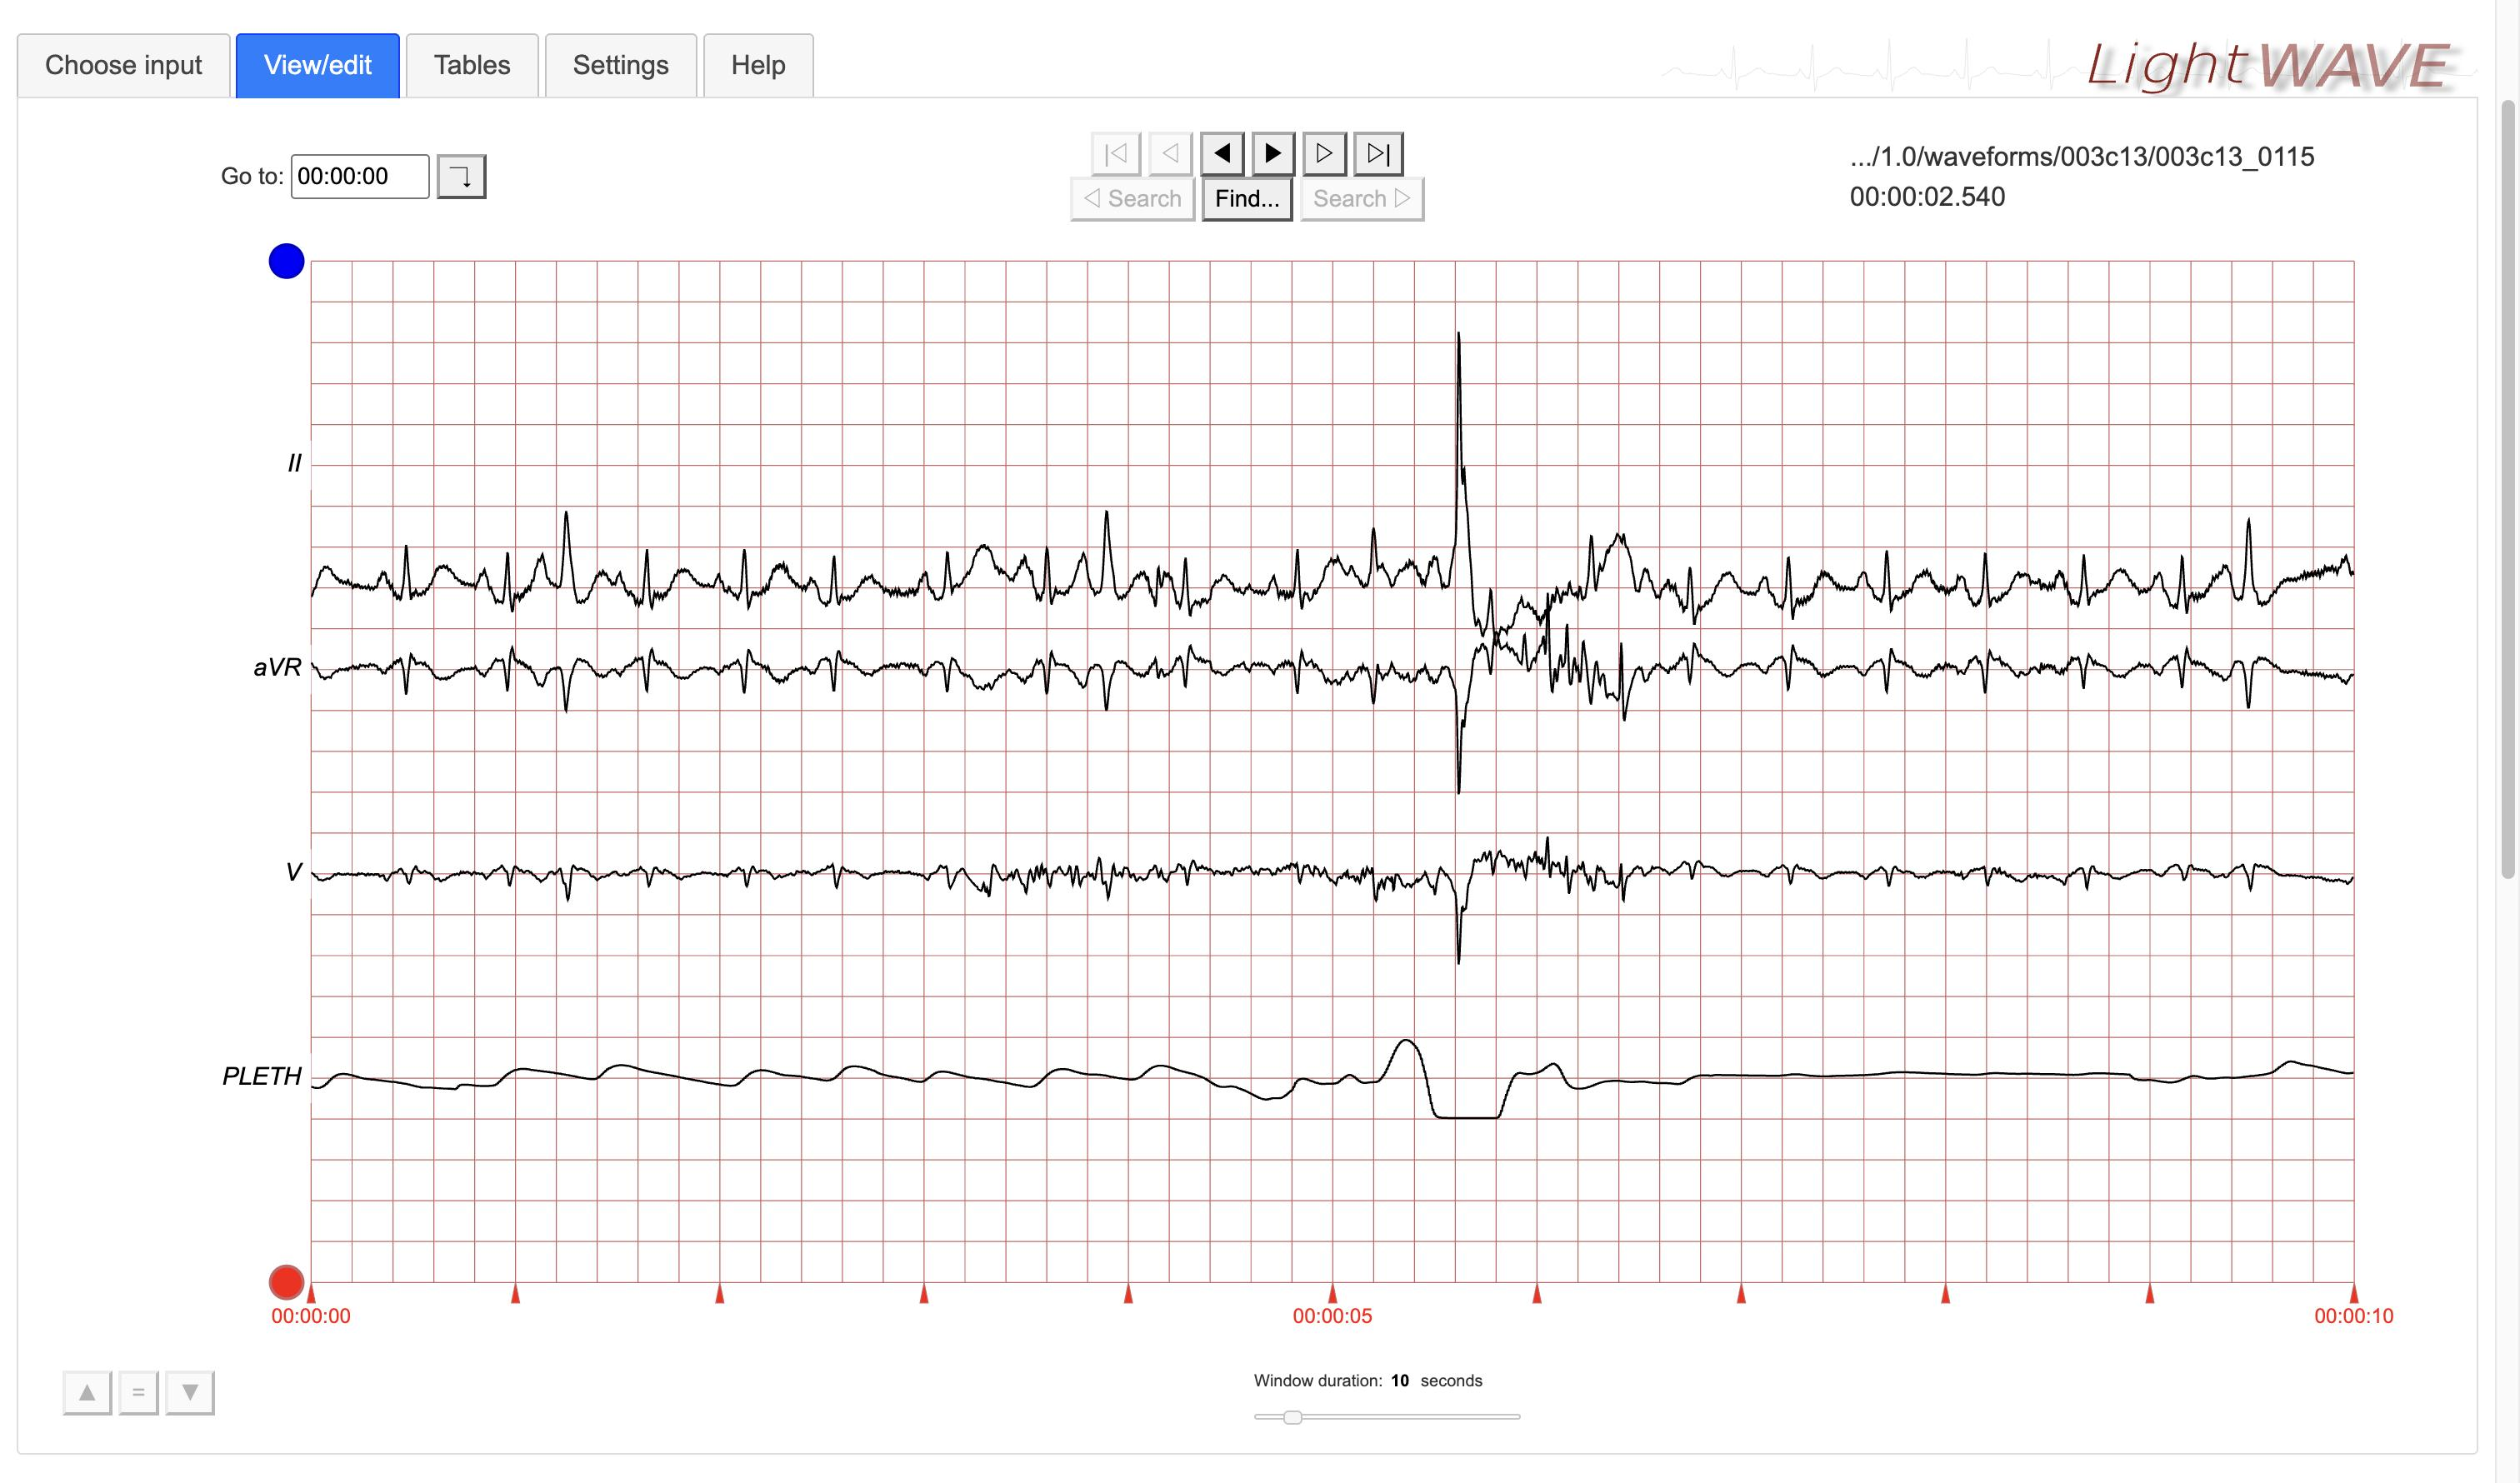
\includegraphics[
        width=\linewidth,
        height=0.32\textheight,
        keepaspectratio
      ]{../images/icu-vital-signs.jpg}

      \small ICU monitoring \citep{PhysioNet-vtac-1.0}
    \end{column}
  \end{columns}
\end{frame}

% \begin{frame}
%   \frametitle{Closely-related publications}
%   \begin{itemize}
%   \item \citep{pei2022transformer} introduced types of attention mechanisms using a re-parametrization trick previously introduced in \citep{jang2017categorical}.
%   \item \citep{Kim_Park_Choo_2024} proposed a detrending-based method to learn new normalities. Then, \citep{park2026paano} suggested using codebook to store normalities, being updated during test-time.
%   \item \citep{Kim_Mok_Lee_Shin_Yoon_2026} experimented finding and using potential false positives to perform light-weight residual update.
%   \end{itemize}
% \end{frame}


% \begin{frame}
%   \frametitle{Limitations of recent methods}
%   \begin{itemize}
%   \item Generally, neural networks can be \textbf{overconfident}, and unable to adapt \textbf{efficiently} when input distribution changes.
%   \item Neural networks in TSAD are not exceptional.
%   \item These 2 limitations remain underexplored.
%   \end{itemize}
% \end{frame}

\begin{frame}
  \frametitle{Related literatures and research gaps}
  \begin{itemize}
  \item Generally, neural networks can be \textbf{overconfident}, and unable to adapt \textbf{efficiently} when input distribution changes.
  \item Neural networks in TSAD are not exceptional.
  \item These 2 limitations remain underexplored.
  \end{itemize}
\end{frame}

\section{Methodologies}

\begin{frame}
    \frametitle{THESIS framework}
    \begin{figure}[H]
    \centering
    \includesvg[width=0.9\linewidth]{../images/thesis-framework.drawio.svg}
    \caption[2 phases of THESIS framework] {2 phases of THESIS framework}
    \label{fig:thesis-framework}
    \end{figure}
\end{frame}

% \begin{frame}
%     \frametitle{Offline phase}
%     \framesubtitle{Offline phase has 2 sequential stages.}
%     \begin{figure}[H]
%     \centering
%     \includesvg[width=0.45\linewidth]{../images/offline-stages.drawio.svg}
%     \caption[Neural network architecture in offline phase] {Neural network architecture in offline phase}
%     \label{fig:offline-architecture}
%     \end{figure}
% \end{frame}

\begin{frame}
    \frametitle{Offline stage A: Multi-task representation learning}
    \framesubtitle{Learning representation for both classification and reconstruction.}
    \begin{figure}[H]
    \centering
    \includesvg[width=0.9\linewidth]{../images/offline-stage-A.drawio.svg}
    \caption[Offline stage A pipeline] {Pipeline of multi-task representation learning process.}
    \label{fig:offline-stage-A}
    \end{figure}
\end{frame}

\begin{frame}
    \frametitle{Memory banks initialization}
    \framesubtitle{Init memory banks using K-Means algorithm.}
    \begin{figure}
        \centering
        \includesvg[width=0.9\linewidth]{../images/banks-init.svg}
        \caption{Initialize memory banks using K-Means clustering algorithm.}
        \label{fig:banks-init}
    \end{figure}
\end{frame}

\begin{frame}
    \frametitle{Offline stage B training: Fusion heads fine-tuning}
    \begin{figure}[H]
    \centering
    \includesvg[width=0.9\linewidth]{../images/offline-stage-B.drawio.svg}
    \caption[Fusion heads fine-tuning pipeline] {Pipeline of fusion heads fine-tuning process.}
    \label{fig:offline-stage-B}
    \end{figure}
\end{frame}

\begin{frame}
    \frametitle{Offline stage B inference: uncertainty estimation}
    \begin{figure}
        \centering
        \includesvg[width=0.9\linewidth]{../images/uncertainty-estimation.svg}
        \caption[Uncertainty estimation] {Uncertainty estimation}
        \label{fig:uncertainty-estimation}
    \end{figure}
\end{frame}

\begin{frame}
    \frametitle{Online test-time adaptation phase}
    \begin{figure}[H]
    \centering
    \includesvg[width=0.8\linewidth]{../images/online-phase.drawio.svg}
    \caption[Online phase pipeline] {Pipeline of online phase with test-time adaptation.}
    \label{fig:online-phase}
    \end{figure}
\end{frame}

% \begin{frame}
%     \frametitle{Offline architecture}
%     \begin{figure}[H]
%     \centering
%     \includesvg[width=0.9\linewidth]{../images/architecture-thesis.drawio.svg}
%     \caption[Neural network architecture in offline phase] {Neural network architecture in offline phase}
%     \label{fig:offline-architecture}
%     \end{figure}
% \end{frame}

% \begin{frame}
%     \frametitle{Multi-task pre-train stage}
%     \begin{figure}[H]
%     \centering
%     \includesvg[width=0.9\linewidth]{../images/pretrain-stage-arch.drawio.svg}
%     \caption[Architecture in pre-train stage] {Neural network architecture in multi-task pre-train stage}
%     \label{fig:pre-train-stage-arch}
%     \end{figure}
% \end{frame}

% \begin{frame}
%     \frametitle{Fusion fine-tuning stage}
%     \begin{figure}[H]
%     \centering
%     \includesvg[width=0.9\linewidth]{../images/fine-tune-stage-arch.drawio.svg}
%     \caption[Architecture in fusion fine-tuning stage] {Neural network architecture in fusion fine-tuning stage}
%     \label{fig:fine-tune-stage-arch}
%     \end{figure}
% \end{frame}

% 

\section{Experimental results}

\begin{frame}
    \frametitle{Offline performance comparison}
    \framesubtitle{SMD entities: machine-1-6, machine-3-4, and machine-3-9}

    \centering
    \tiny
    \setlength{\tabcolsep}{1.8pt}
    \renewcommand{\arraystretch}{0.96}

    \resizebox{\textwidth}{!}{%
    \begin{tabular}{lcccccccccccc}
        \toprule
        \multirow{2}{*}{Method}
        & \multicolumn{3}{c}{machine-1-6}
        & \multicolumn{3}{c}{machine-3-4}
        & \multicolumn{3}{c}{machine-3-9}
        & \multicolumn{3}{c}{Average} \\

        \cmidrule(lr){2-4}
        \cmidrule(lr){5-7}
        \cmidrule(lr){8-10}
        \cmidrule(lr){11-13}

        & VUS-PR & Aff.\ F1 & VUS-ROC
        & VUS-PR & Aff.\ F1 & VUS-ROC
        & VUS-PR & Aff.\ F1 & VUS-ROC
        & VUS-PR & Aff.\ F1 & VUS-ROC \\
        \midrule

        THESIS O0
        & \underline{0.798} & \underline{0.747} & \textbf{0.892}
        & \textbf{0.705} & \underline{0.708} & \textbf{0.950}
        & \underline{0.578} & 0.789 & \underline{0.645}
        & \textbf{0.694} & \underline{0.748} & \underline{0.829} \\

        THESIS O1
        & \textbf{0.799} & \textbf{0.748} & \underline{0.892}
        & \underline{0.705} & 0.708 & \underline{0.950}
        & \underline{0.578} & \underline{0.793} & \underline{0.645}
        & \textbf{0.694} & \textbf{0.749} & \underline{0.829} \\

        RedLamp
        & 0.586 & 0.701 & 0.500
        & 0.614 & \textbf{0.708} & 0.890
        & 0.518 & \textbf{0.824} & 0.547
        & 0.573 & 0.744 & 0.646 \\

        iForest
        & 0.265 & 0.434 & 0.623
        & 0.154 & 0.151 & 0.830
        & 0.028 & 0.645 & 0.249
        & 0.149 & 0.410 & 0.568 \\

        KMeans-AD
        & 0.300 & 0.300 & 0.766
        & 0.392 & 0.136 & 0.949
        & \textbf{0.675} & 0.699 & \textbf{0.900}
        & 0.455 & 0.379 & \textbf{0.872} \\

        StumPy
        & 0.175 & 0.190 & 0.499
        & 0.058 & 0.624 & 0.506
        & 0.045 & 0.592 & 0.550
        & 0.093 & 0.469 & 0.518 \\

        \bottomrule
    \end{tabular}%
    }

    \vspace{0.05em}
    \scriptsize
    $O0$: w/o BPSL; \qquad $O1$: w/ BPSL.

    \vspace{0.15em}

    \scriptsize
    \textbf{Bold}: best
    \qquad
    \underline{Underline}: second best

    \vspace{-0.25em}

    \begin{exampleblock}{Conclusion}
        \scriptsize
        \begin{itemize}
            \setlength{\itemsep}{0.1em}
            \item THESIS leads the baselines on average
                  \textbf{VUS-PR} and \textbf{Aff.\ F1}.
            \item O1 brings little improvement over O0,
                  suggesting a larger contribution from the
                  \textbf{memory modules} than from the balanced loss.
        \end{itemize}
    \end{exampleblock}

\end{frame}

\begin{frame}
    \frametitle{Uncertainty quantification results}
    \framesubtitle{Detection performance and uncertainty across SMD entities}

    \centering
    \tiny
    \setlength{\tabcolsep}{1.4pt}
    \renewcommand{\arraystretch}{0.90}

    \textbf{Per-entity results}

    \resizebox{\textwidth}{!}{%
    \begin{tabular}{lccccccccccccc}
        \toprule
        \multirow{2}{*}{Method}
        & \multirow{2}{*}{BPSL}
        & \multicolumn{4}{c}{machine-1-6}
        & \multicolumn{4}{c}{machine-3-4}
        & \multicolumn{4}{c}{machine-3-9} \\

        \cmidrule(lr){3-6}
        \cmidrule(lr){7-10}
        \cmidrule(lr){11-14}

        & & VUS-PR & Aff.\ F1 & Validation & Test
        & VUS-PR & Aff.\ F1 & Validation & Test
        & VUS-PR & Aff.\ F1 & Validation & Test \\
        \midrule

        THESIS O0
        & -- & 0.798 & 0.747 & 0.012 & 0.250
        & 0.705 & 0.708 & 0.013 & 0.432
        & 0.578 & 0.789 & 0.013 & 0.045 \\

        THESIS O1
        & \checkmark & 0.799 & 0.748 & 0.006 & 0.089
        & 0.704 & 0.708 & 0.019 & 0.573
        & 0.578 & 0.793 & 0.024 & 0.061 \\

    \bottomrule
    \end{tabular}%
    }

    \vspace{0.05em}
    \scriptsize
    BPSL = Balanced Point-Score Loss; \qquad
    $O0$: w/o BPSL; \qquad $O1$: w/ BPSL.

    \vspace{0.15em}

    \begin{columns}[T,onlytextwidth]
        \begin{column}{0.47\textwidth}
            \begin{block}{Average}
                \tiny
                \centering
                \setlength{\tabcolsep}{2.8pt}
                \renewcommand{\arraystretch}{0.90}

                \begin{tabular}{lcccc}
                    \toprule
                    Method & VUS-PR & Aff.\ F1 & Val. & Test \\
                    \midrule
                    O0 & \textbf{0.694} & 0.748 & \textbf{0.013} & \textbf{0.242} \\
                    O1 & \textbf{0.694} & \textbf{0.749} & 0.016 & 0.241 \\
                    \bottomrule
                \end{tabular}
            \end{block}
        \end{column}

        \begin{column}{0.50\textwidth}
            \begin{exampleblock}{Conclusion}
                \scriptsize
                \begin{itemize}
                    \setlength{\itemsep}{0.1em}
                    \item Uncertainty is
                    \textbf{lower on validation}
                    than on test.
                    \item Detection remains strong despite
                    \textbf{higher test uncertainty}.
                    \item This suggests
                    \textbf{generalization without overconfidence}.
                \end{itemize}
            \end{exampleblock}
        \end{column}
    \end{columns}

\end{frame}

\begin{frame}
    \frametitle{Online performance comparison}
    \framesubtitle{THESIS compared with M2N2 and CANDI}

    \centering
    \tiny
    \setlength{\tabcolsep}{1.35pt}
    \renewcommand{\arraystretch}{0.88}

    \resizebox{\textwidth}{!}{%
    \begin{tabular}{lcccccccccccc}
        \toprule
        \multirow{2}{*}{Method}
        & \multicolumn{3}{c}{machine-1-6}
        & \multicolumn{3}{c}{machine-3-4}
        & \multicolumn{3}{c}{machine-3-9}
        & \multicolumn{3}{c}{Average} \\

        \cmidrule(lr){2-4}
        \cmidrule(lr){5-7}
        \cmidrule(lr){8-10}
        \cmidrule(lr){11-13}

        & VUS-PR & Aff.\ F1 & VUS-ROC
        & VUS-PR & Aff.\ F1 & VUS-ROC
        & VUS-PR & Aff.\ F1 & VUS-ROC
        & VUS-PR & Aff.\ F1 & VUS-ROC \\
        \midrule

        THESIS O0 + A0
        & \underline{0.808} & \underline{0.999} & 0.895
        & 0.980 & \textbf{0.721} & 0.978
        & 0.659 & 0.765 & 0.730
        & 0.816 & \underline{0.828} & 0.868 \\

        THESIS O0 + A1
        & \underline{0.808} & \underline{0.999} & 0.895
        & 0.980 & \textbf{0.721} & 0.978
        & 0.659 & 0.765 & 0.730
        & 0.816 & \underline{0.828} & 0.868 \\

        THESIS O0 + A2
        & \underline{0.808} & \underline{0.999} & 0.895
        & 0.980 & \textbf{0.721} & 0.978
        & 0.657 & 0.765 & 0.728
        & 0.815 & \underline{0.828} & 0.867 \\

        \addlinespace[0.1em]

        THESIS O1 + A0
        & \textbf{0.824} & \textbf{0.999} & \underline{0.898}
        & \textbf{0.980} & \textbf{0.721} & 0.977
        & \textbf{0.667} & \underline{0.818} & \underline{0.734}
        & \textbf{0.824} & \textbf{0.846} & 0.869 \\

        THESIS O1 + A1
        & \textbf{0.824} & \textbf{0.999} & \underline{0.898}
        & \textbf{0.980} & \textbf{0.721} & 0.977
        & \textbf{0.667} & \underline{0.818} & \underline{0.734}
        & \textbf{0.824} & \textbf{0.846} & 0.869 \\

        THESIS O1 + A2
        & \textbf{0.824} & \textbf{0.999} & \underline{0.898}
        & \underline{0.980} & \textbf{0.721} & 0.977
        & \underline{0.666} & \underline{0.818} & 0.734
        & \underline{0.824} & \textbf{0.846} & 0.869 \\

        \midrule

        M2N2
        & 0.574 & 0.791 & \textbf{0.983}
        & 0.815 & \textbf{0.721} & \underline{0.976}
        & \textbf{0.717} & \textbf{0.997} & \underline{0.857}
        & 0.702 & \underline{0.836} & \textbf{0.939} \\

        CANDI
        & \underline{0.590} & \underline{0.793} & \underline{0.973}
        & \underline{0.919} & \textbf{0.721} & 0.962
        & 0.608 & 0.808 & \textbf{0.871}
        & \underline{0.706} & 0.774 & \underline{0.935} \\

        \bottomrule
    \end{tabular}%
    }

    \vspace{0.1em}

    \scriptsize
    \textbf{Bold}: best
    \qquad
    \underline{Underline}: second best

    \vspace{-0.25em}

    \begin{exampleblock}{Conclusion}
        \scriptsize
        \begin{itemize}
            \setlength{\itemsep}{0.05em}
            \item Online THESIS achieves higher main detection metrics
                  than the offline-only variants and the baselines.
            \item A0, A1, and A2 differ only marginally,
                  suggesting that \textbf{EWMA score smoothing}
                  contributes most of the online gain.
        \end{itemize}
    \end{exampleblock}

\end{frame}

\begin{frame}
    \frametitle{Conclusions and future directions}
    \framesubtitle{Main findings and next research steps}

    % =========================================================
    % Top summary
    % =========================================================
    \begin{block}{Conclusions}
        \scriptsize
        \vspace{-0.35em}

        \begin{itemize}
            \setlength{\itemsep}{0.15em}

            \item Proposed two retrieval operators:
            \textbf{continuous} and \textbf{discrete},
            together with their \textbf{stochastic variants}
            for uncertainty quantification.

            \item Proposed an \textbf{online test-time adaptation} method
            using a \textbf{triage mechanism} and an
            \textbf{online-to-source contrastive loss}.

            \item Experiments show that both the
            \textbf{offline phase} and the
            \textbf{online phase}
            outperform the selected baselines.

            \item In the online phase,
            \textbf{score smoothing contributes most}
            to the observed performance gain.

            \item Uncertainty is \textbf{higher on test data}
            than on validation data, while the performance metrics still suggest
            \textbf{good generalization} to unseen data.
        \end{itemize}

        \vspace{-0.35em}
    \end{block}

    \vspace{-0.5em}

    % =========================================================
    % Bottom row
    % =========================================================
    \begin{columns}[T,onlytextwidth]

        % ---------- Future direction 1 ----------
        \begin{column}{0.48\textwidth}
            \begin{exampleblock}{Future direction 1}
                \scriptsize
                \vspace{-0.35em}

                \textbf{Reduce false positive rate}
                to alleviate
                \textbf{alarm fatigue},
                especially in domains such as:
                \begin{itemize}
                    \setlength{\itemsep}{0.1em}
                    \item software and cloud system monitoring,
                    \item intensive care units.
                \end{itemize}

                \vspace{-0.35em}
            \end{exampleblock}
        \end{column}

        % ---------- Future direction 2 ----------
        \begin{column}{0.48\textwidth}
            \begin{exampleblock}{Future direction 2}
                \scriptsize
                \vspace{-0.35em}

                Study how to
                \textbf{evaluate the quality of uncertainty estimates},
                so that different uncertainty-quantification methods
                can be compared
                \textbf{fairly}
                in multivariate time-series anomaly detection.

                \vspace{-0.35em}
            \end{exampleblock}
        \end{column}

    \end{columns}

\end{frame}


% \begin{frame}
%   \begin{center}
%     \vfill
%     {\LARGE Contact us to benchmark your model!}
%     \vfill
%     {\LARGE \texttt{forecastbench@forecastingresearch.org}}
%     \vfill
%     {\LARGE \href{https://www.forecastbench.org/}{\texttt{https://www.forecastbench.org}}}
%     \vfill
%   \end{center}
%   \vfill
%   \begin{columns}[T]
%     \column{0.2\textwidth}
%     \column{0.09\textwidth}

%     \ccbysa
%     \column{0.71\textwidth}
%     \tiny
%     Copyright © 2024-2025 Forecasting Research Institute \\
%     License: \href{http://creativecommons.org/licenses/by-sa/4.0/}{Creative
%       Commons Attribution-ShareAlike 4.0}
%   \end{columns}
% \end{frame}

\begin{frame}[allowframebreaks]{References}
    \bibliographystyle{plainnat}
    \bibliography{references}
\end{frame}

% \begin{frame}
%     \frametitle{Deterministic retrieval operators and memory banks}
%     \begin{itemize}
%     \item Given $X_t$, or in short, $X \in \mathbb{R}^{L \times C}$ is an input window inside a batch of samples.
%     \item Raw values of each time-point form a column vector.
%     \end{itemize}
%     \begin{equation}\notag
%     \mathbf{X} = 
%     \begin{bmatrix}
%     x_{0,0} & x_{0,1} & \cdots & x_{0,C-2} & x_{0,C-1} \\
%     x_{1,0} & x_{1,0} & \cdots & x_{1,C-2} & x_{1,C-1} \\
%     \vdots & \vdots & \ddots & \vdots & \vdots \\
%     x_{L-1,0} & x_{L-1,1} & \cdots & x_{L-1,C-2} & x_{L-1,C-1}
%     \end{bmatrix}
%     =
%     \begin{bmatrix}
%     \text{------} & \boldsymbol{x}_0^{\mathsf T} & \text{------} \\
%     \text{------} & \boldsymbol{x}_1^{\mathsf T} & \text{------} \\
%      & \vdots & \\
%     \text{------} & \boldsymbol{x}_{L-1}^{\mathsf T} & \text{------} \\
%     \end{bmatrix}
%     \in \mathbb{R}^{L \times C}
%     \end{equation}

%     \begin{itemize}
%     \item Calculate latent tensor $Z \in \mathbb{R}^{L \times H}$ with all $z_{i}$ has L2-norm equal to 1.
%     \item H is number of dimensions of latent vector space, which is a \textbf{unit hypersphere manifold}.
%     \end{itemize}
%     \begin{equation}\notag
%     \mathbf{Z} = f_{\mathrm{enc}}(\mathbf{X}_t;\boldsymbol{\theta}_{\mathrm{enc}})
%     =
%     \begin{bmatrix}
%     \text{------} & \boldsymbol{z}_0^{\mathsf T} & \text{------} \\
%     \text{------} & \boldsymbol{z}_1^{\mathsf T} & \text{------} \\
%      & \vdots & \\
%     \text{------} & \boldsymbol{z}_{L-1}^{\mathsf T} & \text{------} \\
%     \end{bmatrix}
%     \in \mathbb{R}^{L \times H}
%     \end{equation}
% \end{frame}

% \begin{frame}
%     \frametitle{Continuous prototype bank and discrete codebook}
%     \begin{itemize}
%     \item Let $P^{(c)} \in \mathbb{R}^{K_{c} \times H}$ contains prototypes queried by \textbf{continuous retrieval operator}.
%     \item Let $P^{(d)} \in \mathbb{R}^{K_{d} \times H}$ contains prototypes queried by \textbf{discrete retrieval operator}.
%     \item With branch $b$ can be continuous $c$ or discrete $d$, two memory banks have the same form.
%     \item In code, we set $K_c = 32$ and $K_d = 60$.
%     \end{itemize}
%     \begin{equation}\notag
%     \mathbf{P}^{(b)}
%     =
%     \begin{bmatrix}
%     \text{------} & {\boldsymbol{p}_0^{(b)}}^{\mathsf T} & \text{------} \\
%     \text{------} & {\boldsymbol{p}_1^{(b)}}^{\mathsf T} & \text{------} \\
%      & \vdots & \\
%     \text{------} & {\boldsymbol{p}_{K_{b}-1}^{(b)}}^{\mathsf T} & \text{------} \\
%     \end{bmatrix}
%     \in \mathbb{R}^{K_{b} \times H}
%     \end{equation}
% \end{frame}

% \begin{frame}
%     \frametitle{Continuous deterministic retrieval}
%     \framesubtitle{Dense retrieval from the continuous prototype memory}

%     \begin{block}{1. Match with the continuous memory}
%         \scriptsize
%         \vspace{-0.3em}

%         \begin{columns}[c,onlytextwidth]

%             \begin{column}{0.34\textwidth}
%                 \textbf{Memory}

%                 \[
%                 \mathbf{P}^{(c)}
%                 \in \mathbb{R}^{K_c\times H}
%                 \]

%                 $K_c$ learned normal prototypes.
%             \end{column}

%             \begin{column}{0.62\textwidth}
%                 \textbf{Similarity weights}

%                 \[
%                 \alpha^{(c)}_{i,k}
%                 =
%                 \operatorname{softmax}_k
%                 \left(
%                     \frac{
%                         \mathbf{z}_i^\top\mathbf{p}^{(c)}_k
%                     }{\tau_c}
%                 \right),
%                 \qquad \tau_c>0
%                 \]

%                 Higher similarity $\Rightarrow$ larger weight.
%             \end{column}

%         \end{columns}

%         \vspace{-0.2em}
%     \end{block}

%     \vspace{-0.5em}

%     \begin{exampleblock}{2. Build the continuous-branch representation}
%         \scriptsize
%         \vspace{-0.3em}

%         \begin{columns}[c,onlytextwidth]

%             \begin{column}{0.47\textwidth}
%                 \centering

%                 \[
%                 \widetilde{\mathbf{z}}^{(c)}_i
%                 =
%                 \sum_{k=1}^{K_c}
%                 \alpha^{(c)}_{i,k}
%                 \mathbf{p}^{(c)}_k
%                 \]

%                 \textbf{continuous-branch latent vector}
%             \end{column}

%             \begin{column}{0.49\textwidth}
%                 \textbf{Interpretation}

%                 \textbf{Dense retrieval:}
%                 all $K_c$ prototypes contribute.

%                 \vspace{0.15em}

%                 Cross-attention-like,
%                 but without residual addition.
%             \end{column}

%         \end{columns}

%         \vspace{-0.2em}
%     \end{exampleblock}

% \end{frame}

% \begin{frame}
%     \frametitle{Discrete deterministic retrieval}
%     \framesubtitle{Sparse retrieval from the discrete prototype memory}

%     \begin{block}{1. Find the nearest codewords}
%         \scriptsize
%         \vspace{-0.4em}

%         \begin{columns}[c,onlytextwidth]

%             \begin{column}{0.45\textwidth}
%                 \textbf{Distance}

%                 \[
%                 d^{(d)}_{i,k}
%                 =
%                 \left\|
%                     \mathbf{z}_i-\mathbf{p}^{(d)}_k
%                 \right\|_2^2
%                 \]

%                 For unit-normalized vectors:
%                 \[
%                 d^{(d)}_{i,k}
%                 =
%                 2\bigl(
%                     1-\cos(
%                     \mathbf{z}_i,\mathbf{p}^{(d)}_k)
%                 \bigr)
%                 \]
%             \end{column}

%             \begin{column}{0.51\textwidth}
%                 \textbf{Top-$K$ selection}

%                 \[
%                 \mathcal{I}^{(d)}_i
%                 =
%                 \operatorname{TopKMin}_{k}
%                 \left(
%                     d^{(d)}_{i,k};
%                     K_{\mathrm{top}}
%                 \right)
%                 \]

%                 Keep only the nearest
%                 $K_{\mathrm{top}}=3$ codewords.
%             \end{column}

%         \end{columns}

%         \vspace{-0.35em}
%     \end{block}

%     \vspace{-0.55em}

%     \begin{exampleblock}{2. Weight and retrieve}
%         \scriptsize
%         \vspace{-0.4em}

%         \begin{columns}[c,onlytextwidth]

%             \begin{column}{0.48\textwidth}
%                 \centering

%                 \[
%                 \alpha^{(d)}_{i,k}
%                 =
%                 \operatorname{softmax}_{
%                     k\in\mathcal{I}^{(d)}_i}
%                 \left(
%                     -\frac{d^{(d)}_{i,k}}{\tau_d}
%                 \right)
%                 \]

%                 closer $\Rightarrow$ larger weight
%             \end{column}

%             \begin{column}{0.48\textwidth}
%                 \centering

%                 \[
%                 \widetilde{\mathbf{z}}^{(d)}_i
%                 =
%                 \sum_{k\in\mathcal{I}^{(d)}_i}
%                 \alpha^{(d)}_{i,k}
%                 \mathbf{p}^{(d)}_k
%                 \]

%                 \textbf{discrete-branch latent vector}

%                 \textbf{Sparse:} only Top-$K$ contributes.
%             \end{column}

%         \end{columns}

%         \vspace{-0.35em}
%     \end{exampleblock}

% \end{frame}

% \begin{frame}
%     \frametitle{Continuous stochastic retrieval}
%     \framesubtitle{Stochastic dense retrieval for epistemic uncertainty}

%     \begin{block}{1. Perturb the continuous retrieval}
%         \scriptsize
%         \vspace{-0.3em}

%         \begin{columns}[c,onlytextwidth]

%             \begin{column}{0.32\textwidth}
%                 \textbf{Gumbel noise}

%                 \[
%                 g^{(c,m)}_{i,k}
%                 \sim
%                 \operatorname{Gumbel}(0,1)
%                 \]

%                 New perturbation for draw $m$.
%             \end{column}

%             \begin{column}{0.64\textwidth}
%                 \textbf{Stochastic weights}

%                 \[
%                 \alpha^{(c,m)}_{i,k}
%                 =
%                 \operatorname{softmax}_k
%                 \left(
%                     \frac{
%                         \mathbf{z}_i^\top\mathbf{p}^{(c)}_k
%                         +g^{(c,m)}_{i,k}
%                     }{\tau_c}
%                 \right)
%                 \]

%                 All $K_c$ prototypes remain eligible.
%             \end{column}

%         \end{columns}

%         \vspace{-0.2em}
%     \end{block}

%     \vspace{-0.5em}

%     \begin{exampleblock}{2. Build a stochastic continuous representation}
%         \scriptsize
%         \vspace{-0.3em}

%         \begin{columns}[c,onlytextwidth]

%             \begin{column}{0.47\textwidth}
%                 \centering

%                 \[
%                 \widetilde{\mathbf{z}}^{(c,m)}_i
%                 =
%                 \sum_{k=1}^{K_c}
%                 \alpha^{(c,m)}_{i,k}
%                 \mathbf{p}^{(c)}_k
%                 \]

%                 one representation for draw $m$
%             \end{column}

%             \begin{column}{0.49\textwidth}
%                 \textbf{Interpretation}

%                 \textbf{Dense:}
%                 all prototypes can contribute.

%                 \vspace{0.15em}

%                 Different draws produce different
%                 soft mixtures, supporting
%                 \textbf{epistemic uncertainty estimation}.
%             \end{column}

%         \end{columns}

%         \vspace{-0.2em}
%     \end{exampleblock}

% \end{frame}

% \begin{frame}
%     \frametitle{Discrete stochastic retrieval}
%     \framesubtitle{Stochastic sparse retrieval from the discrete memory}

%     \begin{block}{1. Perturb and select the neighborhood}
%         \scriptsize
%         \vspace{-0.3em}

%         \begin{columns}[c,onlytextwidth]

%             \begin{column}{0.45\textwidth}
%                 \textbf{Stochastic score}

%                 \[
%                 q^{(d,m)}_{i,k}
%                 =
%                 \frac{
%                     -d^{(d)}_{i,k}
%                     +g^{(d,m)}_{i,k}
%                 }{\tau_d}
%                 \]

%                 \[
%                 g^{(d,m)}_{i,k}
%                 \sim
%                 \operatorname{Gumbel}(0,1)
%                 \]
%             \end{column}

%             \begin{column}{0.51\textwidth}
%                 \textbf{Stochastic Top-$K$}

%                 \[
%                 \mathcal{I}^{(d,m)}_i
%                 =
%                 \operatorname{TopKMax}_{k}
%                 \left(
%                     q^{(d,m)}_{i,k};
%                     K_{\mathrm{top}}
%                 \right)
%                 \]

%                 Neighborhood can change with $m$.

%                 \[
%                 K_{\mathrm{top}}=3
%                 \]
%             \end{column}

%         \end{columns}

%         \vspace{-0.2em}
%     \end{block}

%     \vspace{-0.5em}

%     \begin{exampleblock}{2. Weight and retrieve}
%         \scriptsize
%         \vspace{-0.45em}
    
%         \begin{columns}[c,onlytextwidth]
    
%             \begin{column}{0.49\textwidth}
%                 \centering
%                 \textbf{Weights}
    
%                 \[
%                 \alpha^{(d,m)}_{i,k}
%                 =
%                 \operatorname{softmax}_{
%                     k\in\mathcal{I}^{(d,m)}_i}
%                 \left(
%                     q^{(d,m)}_{i,k}
%                 \right)
%                 \]
    
%                 selected codewords only
%             \end{column}
    
%             \begin{column}{0.49\textwidth}
%                 \centering
%                 \textbf{Retrieved representation}
    
%                 \[
%                 \widetilde{\mathbf{z}}^{(d,m)}_i
%                 =
%                 \sum_{k\in\mathcal{I}^{(d,m)}_i}
%                 \alpha^{(d,m)}_{i,k}
%                 \mathbf{p}^{(d)}_k
%                 \]
    
%                 \textbf{stochastic sparse retrieval}
%             \end{column}
    
%         \end{columns}
    
%         \vspace{-0.15em}
    
%         \centering
%         \textbf{Different draws can select different Top-$K$ neighborhoods.}
    
%         \vspace{-0.4em}
%     \end{exampleblock}
% \end{frame}

% \begin{frame}
%     \frametitle{Offline anomaly threshold}
%     \framesubtitle{Calibrate from validation reconstruction errors only.}

%     \begin{block}{Calibration}
%         \scriptsize

%         \begin{columns}[T,onlytextwidth]

%             \begin{column}{0.47\textwidth}
%                 \textbf{Validation scores}

%                 Use non-overlapping validation windows:

%                 \[
%                 s_i
%                 =
%                 \frac{1}{C}
%                 \left\|
%                     \mathbf{x}_i
%                     -
%                     \widehat{\mathbf{x}}_i
%                 \right\|_2^2
%                 \]

%                 Collect all point-level scores:

%                 \[
%                 \mathcal{S}_{\mathrm{val}}
%                 =
%                 \{s_1,\ldots,s_N\}.
%                 \]
%             \end{column}

%             \begin{column}{0.47\textwidth}
%                 \textbf{Threshold}

%                 Calibrate only from validation:

%                 \[
%                 \delta_{\mathrm{pt}}
%                 =
%                 \operatorname{Calibrate}
%                 \left(
%                     \mathcal{S}_{\mathrm{val}}
%                 \right)
%                 \]

%                 Predict:

%                 \[
%                 \widehat{a}_n
%                 =
%                 \mathbb{I}
%                 \left(
%                     s_n>\delta_{\mathrm{pt}}
%                 \right).
%                 \]
%             \end{column}

%         \end{columns}
%     \end{block}

%     \vspace{-0.4em}

%     \begin{exampleblock}{Takeaway}
%         \scriptsize
%         \centering
%         \textbf{Validation only:}
%         no test data are used to choose the threshold.
%     \end{exampleblock}

% \end{frame}

% \section{Online adaptation mechanism}
% \begin{frame}
%     \frametitle{Online adaptation architecture}
%     \begin{figure}[H]
%     \centering
%     \includesvg[width=0.9\linewidth]{../images/online-adaptation-arch.drawio.svg}
%     \caption[Neural network architecture in online phase] {Neural network architecture in online phase}
%     \label{fig:online-architecture}
%     \end{figure}
% \end{frame}

% \begin{frame}
%     \frametitle{Online anomaly score smoothing}
%     \framesubtitle{Average stochastic scores, then smooth repeated observations}

%     % =========================================================
%     % Stochastic score aggregation
%     % =========================================================
%     \begin{block}{1. Aggregate stochastic reconstruction scores}
%         \scriptsize
%         \vspace{-0.3em}

%         \begin{columns}[c,onlytextwidth]

%             % ---------- Per-pass score ----------
%             \begin{column}{0.47\textwidth}
%                 \textbf{Each stochastic pass}

%                 \[
%                 s^{(m)}_{i}
%                 =
%                 \frac{1}{C}
%                 \left\|
%                     \mathbf{x}_{i}
%                     -
%                     \widehat{\mathbf{x}}^{(m)}_{i}
%                 \right\|_2^2
%                 \]

%                 one reconstruction score for pass $m$
%             \end{column}

%             % ---------- Mean score ----------
%             \begin{column}{0.47\textwidth}
%                 \textbf{Average over $M$ passes}

%                 \[
%                 \overline{s}_{i}
%                 =
%                 \frac{1}{M}
%                 \sum_{m=1}^{M}
%                 s^{(m)}_{i}
%                 \]

%                 one mean score for this window occurrence
%             \end{column}

%         \end{columns}

%         \vspace{-0.2em}
%     \end{block}

%     \vspace{-0.5em}

%     % =========================================================
%     % EWMA smoothing
%     % =========================================================
%     \begin{exampleblock}{2. Smooth repeated appearances across sliding windows}
%         \scriptsize
%         \vspace{-0.3em}

%         \begin{columns}[c,onlytextwidth]

%             % ---------- EWMA ----------
%             \begin{column}{0.52\textwidth}
%                 \textbf{EWMA update}

%                 \[
%                 \widetilde{s}^{(r)}_{n}
%                 =
%                 \rho\,\overline{s}^{(r)}_{n}
%                 +
%                 (1-\rho)\widetilde{s}^{(r-1)}_{n}
%                 \]

%                 \[
%                 \rho=0.9
%                 \qquad
%                 \widetilde{s}^{(1)}_n
%                 =
%                 \overline{s}^{(1)}_n
%                 \]

%                 \centering
%                 \textbf{90\% current + 10\% previous}
%             \end{column}

%             % ---------- Meaning + decision ----------
%             \begin{column}{0.44\textwidth}
%                 \textbf{Why?}

%                 A global time point may appear
%                 in multiple sliding windows.

%                 \vspace{0.25em}

%                 $n$: global time-point index

%                 $r$: number of appearances

%                 \vspace{0.35em}

%                 \textbf{Point decision}

%                 \[
%                 \widehat{a}_n
%                 =
%                 \mathbb{I}
%                 \left(
%                     \widetilde{s}_n
%                     >
%                     \delta_{\mathrm{pt}}
%                 \right)
%                 \]
%             \end{column}

%         \end{columns}

%         \vspace{-0.2em}
%     \end{exampleblock}

% \end{frame}

% \begin{frame}
%     \frametitle{Triage operator and verification buffer}
%     \framesubtitle{Route confident cases immediately; verify uncertain cases over time}

%     % =========================================================
%     % TRIAGE
%     % =========================================================
%     \begin{block}{1. Triage each online window}
%         \scriptsize
%         \vspace{-0.35em}

%         \centering
%         \setlength{\tabcolsep}{3.5pt}
%         \renewcommand{\arraystretch}{1.05}

%         \begin{tabular}{lccc}
%             \textbf{Route}
%             & $\mathbf{S^{(\mathrm{input})}}$
%             & $\mathbf{S^{(\mathrm{latent})}}$
%             & \textbf{Action} \\
%             \hline

%             normal
%             & $\leq\delta_{\mathrm{rec}}$
%             & --
%             & no adaptation \\

%             hard-old-normality
%             & $>\delta_{\mathrm{rec}}$
%             & $\leq\delta_{\mathrm{lat}}^{-}$
%             & \textbf{adapt} \\

%             gray zone
%             & $>\delta_{\mathrm{rec}}$
%             & $(\delta_{\mathrm{lat}}^{-},
%                \delta_{\mathrm{lat}}^{+}]$
%             & \textbf{verify} \\

%             strong anomaly
%             & $>\delta_{\mathrm{rec}}$
%             & $>\delta_{\mathrm{lat}}^{+}$
%             & no adaptation
%         \end{tabular}

%         \vspace{-0.25em}
%     \end{block}

%     \vspace{-0.5em}

%     % =========================================================
%     % VERIFICATION
%     % =========================================================
%     \begin{exampleblock}{2. Verify only gray-zone windows}
%         \scriptsize
%         \vspace{-0.35em}

%         \begin{columns}[c,onlytextwidth]

%             \begin{column}{0.23\textwidth}
%                 \centering
%                 \textbf{Buffer}

%                 gray-zone windows

%                 \[
%                 \mathcal{B}
%                 \]
%             \end{column}

%             \begin{column}{0.24\textwidth}
%                 \centering
%                 \textbf{Filter}

%                 remove points in
%                 known anomalous clusters
%             \end{column}

%             \begin{column}{0.25\textwidth}
%                 \centering
%                 \textbf{Verify}

%                 find signatures repeated
%                 across multiple windows
%             \end{column}

%             \begin{column}{0.24\textwidth}
%                 \centering
%                 \textbf{Output}

%                 \[
%                 \mathcal{V}
%                 \]

%                 verified pseudo-new-normality
%             \end{column}

%         \end{columns}

%         \vspace{-0.2em}

%         \centering
%         $\mathcal{V}\neq\varnothing$:
%         \textbf{adapt on verified points}
%         \qquad
%         $\mathcal{V}=\varnothing$:
%         \textbf{unresolved}

%         \vspace{-0.25em}
%     \end{exampleblock}

% \end{frame}

% \begin{frame}
%     \frametitle{Online-to-source contrastive loss}
%     \framesubtitle{Adapt without drifting toward known anomalous representations}

%     % =========================================================
%     % 1. Contrastive roles
%     % =========================================================
%     \begin{block}{1. Contrastive roles}
%         \scriptsize
%         \vspace{-0.45em}
    
%         \begin{columns}[c,onlytextwidth]
    
%             % ---------- Anchor ----------
%             \begin{column}{0.24\textwidth}
%                 \centering
%                 \textbf{Anchor}
    
%                 \[
%                 \boxed{\mathbf z_i^{(\mathrm{on})}}
%                 \]
    
%                 online representation
%             \end{column}
    
%             % ---------- Positive ----------
%             \begin{column}{0.34\textwidth}
%                 \centering
%                 \textbf{Positive}
    
%                 \[
%                 \mathbf z_i^{(\mathrm{src})}
%                 \qquad
%                 \cos(
%                     \mathbf z_i^{(\mathrm{on})},
%                     \mathbf z_i^{(\mathrm{src})}
%                 ) \uparrow
%                 \]
    
%                 \textbf{stay near source}
%             \end{column}
    
%             % ---------- Negatives ----------
%             \begin{column}{0.38\textwidth}
%                 \centering
%                 \textbf{Negatives}
    
%                 \[
%                 \mathbf p_k^{(d)},
%                 \ k\in\mathcal K_{\mathrm{anom}}
%                 \qquad
%                 \cos(
%                     \mathbf z_i^{(\mathrm{on})},
%                     \mathbf p_k^{(d)}
%                 ) \downarrow
%                 \]
    
%                 \textbf{stay away from anomalies}
%             \end{column}
    
%         \end{columns}
    
%         \vspace{-0.4em}
%     \end{block}

%     \vspace{-0.55em}

%     % =========================================================
%     % 2. Adaptation rule
%     % =========================================================
%     \begin{exampleblock}{2. Adaptation rule}
%         \scriptsize
%         \vspace{-0.35em}

%         \begin{columns}[c,onlytextwidth]

%             \begin{column}{0.48\textwidth}
%                 \centering
%                 \textbf{Representation constraint}

%                 \[
%                 \operatorname{sim}
%                 (\mathbf z_i^{(\mathrm{on})},
%                  \mathbf z_i^{(\mathrm{src})})
%                 \uparrow
%                 \qquad
%                 \operatorname{sim}
%                 (\mathbf z_i^{(\mathrm{on})},
%                  \mathbf p_k^{(d)})
%                 \downarrow
%                 \]

%                 preserve source geometry
%             \end{column}

%             \begin{column}{0.48\textwidth}
%                 \centering
%                 \textbf{Update scope}

%                 \[
%                 \boxed{
%                     \boldsymbol{\phi}
%                     \text{ : MLP projector}
%                 }
%                 \]

%                 \textbf{Frozen:}
%                 encoder, memories, fusion, heads
%             \end{column}

%         \end{columns}

%         \vspace{-0.3em}
%     \end{exampleblock}

% \end{frame}

\end{document}
